\documentclass[12pt, paper=a4]{article}
\usepackage[utf8]{inputenc}
\usepackage[german]{babel}
\usepackage{mathrsfs}
\usepackage{amsmath}
\usepackage{amssymb}
\usepackage{listings}
\usepackage{graphicx}
\usepackage{fancyhdr}

\setlength{\parindent}{0pt}

\author{Mareike G\"ottsch, 6695217, Gruppe 2\\Paul H\"olzen, 6673477, Gruppe 1\\Sven Schmidt, 6217064, Gruppe 1}

\title{FGI 2 Hausaufgaben 6}

\rhead{M. G\"ottsch, G-2; P. H\"olzen, G-1; S. Schmidt, G-1}
\pagestyle{fancy}
\begin{document}
\maketitle

\section*{Aufgabe 6.3}


\begin{enumerate}
	\item \(VC(\phi_{01})=(1,0,0,0); VC(\phi_{02})=(2,0,0,0); VC(\phi_{03})=(3,3,1,0);\\
	VC(\phi_{04})=(4,3,1,4); VC(\phi_{05})=(5,3,1,4); VC(\phi_{06})=(6,3,1,4);\\
	VC(\phi_{11})=(1,1,0,0); VC(\phi_{12})=(1,2,1,0); VC(\phi_{13})=(1,3,1,0);\\
	VC(\phi_{14})=(1,4,1,0); VC(\phi_{15})=(5,5,5,4); VC(\phi_{16})=(5,6,5,6);\\
	VC(\phi_{21})=(0,0,1,0); VC(\phi_{22})=(0,0,2,1); VC(\phi_{23})=(2,0,3,3);\\
	VC(\phi_{24})=(5,3,4,4); VC(\phi_{25})=(5,3,5,4); VC(\phi_{26})=(6,3,6,4);\\
	VC(\phi_{31})=(0,0,0,1); VC(\phi_{32})=(2,0,0,2); VC(\phi_{33})=(2,0,0,3);\\
	VC(\phi_{34})=(2,0,0,4); VC(\phi_{35})=(2,4,1,5); VC(\phi_{36})=(2,4,1,6)\)
	
	\item Es gilt: \(\phi_{02}  \textbf{ vor } \phi_{32} \textbf{ vor } \phi_{23} \textbf{ vor } \phi_{15}\)\\
	mit \(VC(\phi_{02})=(2,0,0,0), VC(\phi_{32})=(2,0,0,2), VC(\phi_{23})=(2,0,3,3),\\
	VC(\phi_{15})=(5,5,5,4)\)
	
	\item Betrachte \(\phi_{03}, \phi_{14}, \phi_{22}\) und \(\phi_{32}\). Diese sind paarweise unabh\"angig.\\
	Es gilt:
		\begin{itemize}
			\item \(\phi_{03} || \phi_{14} \Leftrightarrow \lnot (\phi_{03} \textbf{ vor } \phi_{14}) \land  
			\lnot (\phi_{14} \textbf{ vor } \phi_{03})\)
			\item \(\phi_{03} || \phi_{22} \Leftrightarrow \lnot (\phi_{03} \textbf{ vor } \phi_{22}) \land  
			\lnot (\phi_{22} \textbf{ vor } \phi_{03})\)
			\item \(\phi_{03} || \phi_{32} \Leftrightarrow \lnot (\phi_{03} \textbf{ vor } \phi_{32}) \land  
			\lnot (\phi_{32} \textbf{ vor } \phi_{03})\)
			\item \(\phi_{14} || \phi_{22} \Leftrightarrow \lnot (\phi_{14} \textbf{ vor } \phi_{22}) \land  
			\lnot (\phi_{22} \textbf{ vor } \phi_{14})\)
			\item \(\phi_{14} || \phi_{32} \Leftrightarrow \lnot (\phi_{14} \textbf{ vor } \phi_{32}) \land  
			\lnot (\phi_{32} \textbf{ vor } \phi_{14})\)
			\item \(\phi_{22} || \phi_{32} \Leftrightarrow \lnot (\phi_{22} \textbf{ vor } \phi_{32}) \land  
			\lnot (\phi_{32} \textbf{ vor } \phi_{22})\)
		\end{itemize}
	mit den Vektorzeiten: \(VC(\phi_{03})=(3,3,1,0), VC(\phi_{14})=(1,4,1,0),\\
	VC(\phi_{22})=(0,0,2,1)\) und \(VC(\phi_{32})=(2,0,0,2)\).
	
	\item F\"ur diesen Aufgabenteil werden nur Ereignisse betrachtet, welche einen logischen Zeitstempel bis \((3,p_i)\)
	gem\"a{\ss} Lamport-Ordnung haben. Diese sind:\\
	\((LT(\phi_{01}),p_i)=(1,p_0), (LT(\phi_{02}),p_i)=(2,p_0),\\
	(LT(\phi_{11}),p_i)=(2,p_1), (LT(\phi_{12}),p_i)=(3,p_1),\\
	(LT(\phi_{21}),p_i)=(1,p_2), (LT(\phi_{22}),p_i)=(2,p_2),\\
	(LT(\phi_{31}),p_i)=(1,p_3), (LT(\phi_{32}),p_i)=(3,p_3)\).\\
	F\"ur diese Ereignisse gilt:\\
	\(\phi_{01} <_L \phi_{21} <_L \phi_{31} <_L \phi_{02} <_L \phi_{11} <_L \phi_{22} <_L \phi_{12} <_L \phi_{32} \)
	
	\item
	
	\item
\end{enumerate}

\section*{Aufgabe 6.4}
\begin{figure}[h!]
\centering
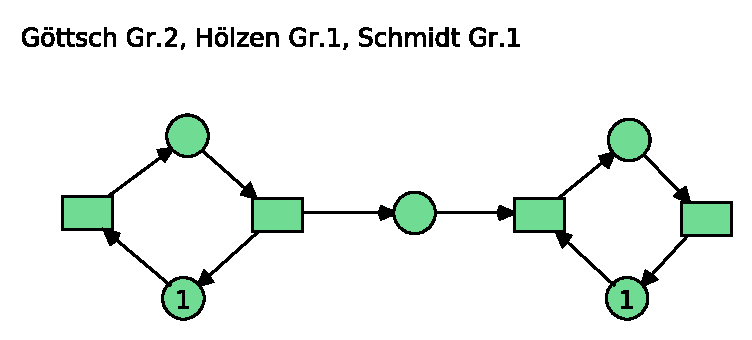
\includegraphics[scale=0.7]{G-1-A-06-OriginalNetz-Goettsch_Hoelzen_Schmidt.pdf}
\caption{Original Netz}
\end{figure}

\begin{figure}[h!]
\centering
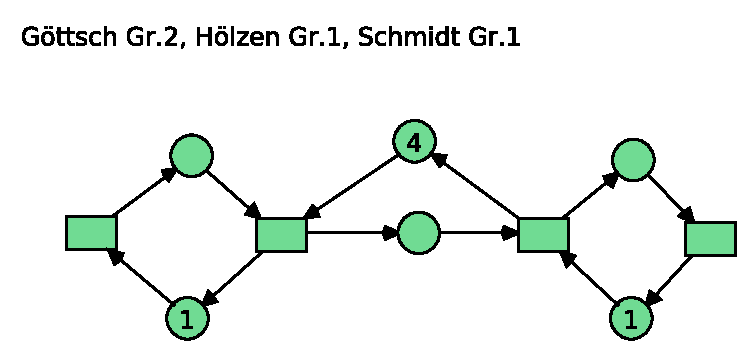
\includegraphics[scale=0.7]{G-1-A-06-Maximum4-Goettsch_Hoelzen_Schmidt.pdf}
\caption{Lager beschränkt auf eine Kapazität von 4 Marken}
\end{figure}

\begin{figure}[h!]
\centering
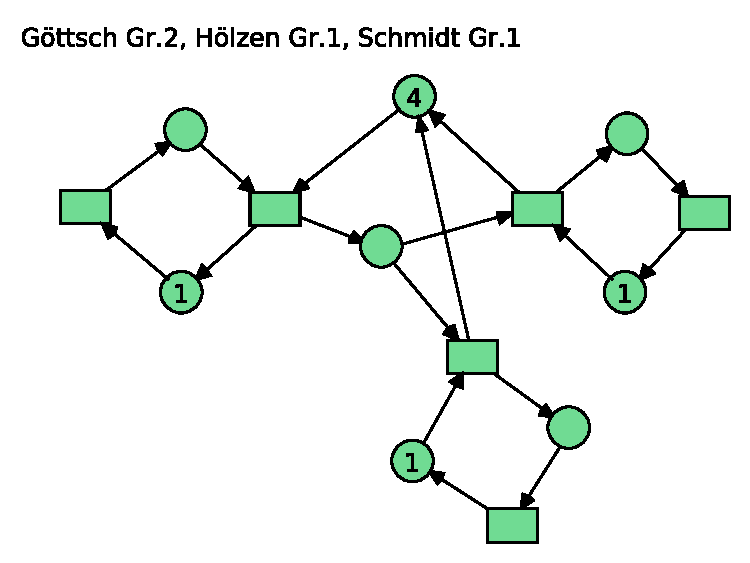
\includegraphics[scale=0.7]{G-1-A-06-ZweiEmpfaenger-Goettsch_Hoelzen_Schmidt.pdf}\caption{Zwei Empfänger}
\end{figure}

\begin{figure}[h!]
\centering
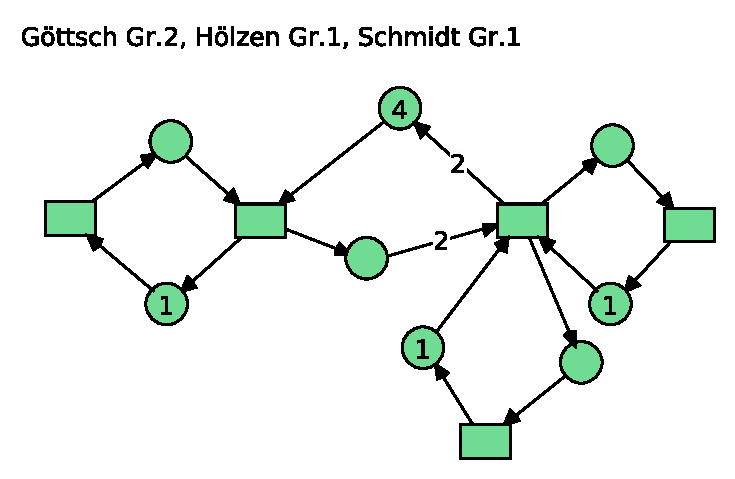
\includegraphics[scale=0.7]{G-1-A-06-ZweiGleichzeitig-Goettsch_Hoelzen_Schmidt.pdf}
\caption{Zwei Nachrichten werden gleichzeitig entnommen}
\end{figure}

\begin{figure}[h!]
\centering
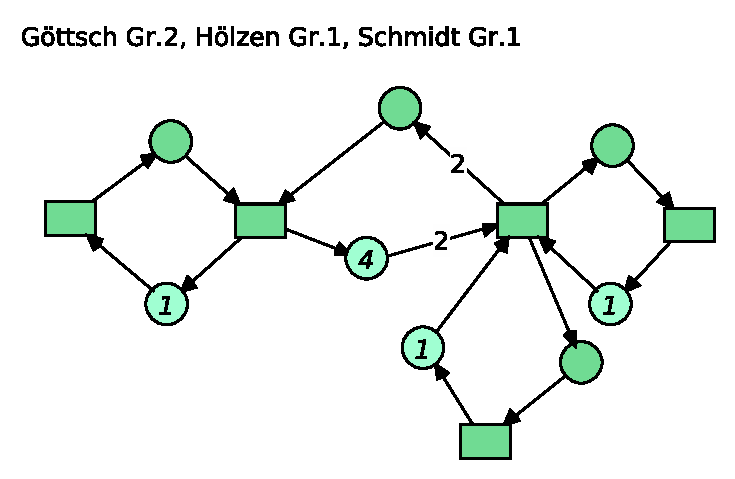
\includegraphics[scale=0.7]{G-1-A-06-ZweiGleichzeitigLagerVollSim-Goettsch_Hoelzen_Schmidt.pdf}
\caption{Simulations-Zustand: Lager voll}
\end{figure}

\end{document}


















